\documentclass[12pt]{article}
\usepackage{times} 			% use Times New Roman font

\usepackage[margin=1in]{geometry}   % sets 1 inch margins on all sides
\usepackage{hyperref}               % for URL formatting
\usepackage[pdftex]{graphicx}       % So includegraphics will work
\setlength{\parskip}{1em}           % skip 1em between paragraphs
\usepackage{indentfirst}            % indent the first line of each paragraph
\usepackage{datetime}
\usepackage[small, bf]{caption}
\usepackage{listings}               % for code listings
\usepackage{xcolor}                 % for styling code
\usepackage{multirow}

%New colors defined below
\definecolor{backcolour}{RGB}{246, 246, 246}   % 0xF6, 0xF6, 0xF6
\definecolor{codegreen}{RGB}{16, 124, 2}       % 0x10, 0x7C, 0x02
\definecolor{codepurple}{RGB}{170, 0, 217}     % 0xAA, 0x00, 0xD9
\definecolor{codered}{RGB}{154, 0, 18}         % 0x9A, 0x00, 0x12

%Code listing style named "gcolabstyle" - matches Google Colab
\lstdefinestyle{gcolabstyle}{
  basicstyle=\ttfamily\small,
  backgroundcolor=\color{backcolour},   
  commentstyle=\itshape\color{codegreen},
  keywordstyle=\color{codepurple},
  stringstyle=\color{codered},
  numberstyle=\ttfamily\footnotesize\color{darkgray}, 
  breakatwhitespace=false,         
  breaklines=true,                 
  captionpos=b,                    
  keepspaces=true,                 
  numbers=left,                    
  numbersep=5pt,                  
  showspaces=false,                
  showstringspaces=false,
  showtabs=false,                  
  tabsize=2
}

\lstset{style=gcolabstyle}      %set gcolabstyle code listing

% to make long URIs break nicely
\makeatletter
\g@addto@macro{\UrlBreaks}{\UrlOrds}
\makeatother

% for fancy page headings
\usepackage{fancyhdr}
\setlength{\headheight}{13.6pt} % to remove fancyhdr warning
\pagestyle{fancy}
\fancyhf{}
\rhead{\small \thepage}
\lhead{\small HW4, Bartels}  % EDIT THIS, REPLACE # with HW number
\chead{\small CS 432, Fall 2020} 

%-------------------------------------------------------------------------
\begin{document}

\begin{centering}
{\large\textbf{HW4 - Exploring Social Networks}}\\ % EDIT THIS
                                % REPLACE # with HW num and ADD title
Logan Bartels\\                     % EDIT THIS
October 25, 2020\\                      % EDIT THIS
\end{centering}

%-------------------------------------------------------------------------

\section*{Note about R scripts}
Most of my R scripts were tested on a copy of the Week-03-InfoVis-R Google Collab notebook.  The png versions of the graphs shown in this report were saved from the Collab notebook.  Some lines of code found in the notebook were omitted in my final R scripts for brevity.  The code can be found under the ``HW4'' section here:\\
\url{https://colab.research.google.com/drive/1BVYc-LunOuLe4bI-1S1xea3nP_lZ_wdH?usp=sharing}

\section*{Q1}



\subsection*{Answer}

\lstinputlisting[caption=Mean standard deviation and median of Facebook friends found in HW4-friend-count.csv., label=facebookData]{facebookData.txt}

\lstinputlisting[language=R, caption=R script used to calculate output in listing \ref{facebookData}., label=calFbData]{friendData.R}

\lstinputlisting[language=R, caption=Rscript used to graph Facebook friends based on their number of friends., label=graphFriends]{graphFriends.R}

\begin{figure}[h]
    \centering
    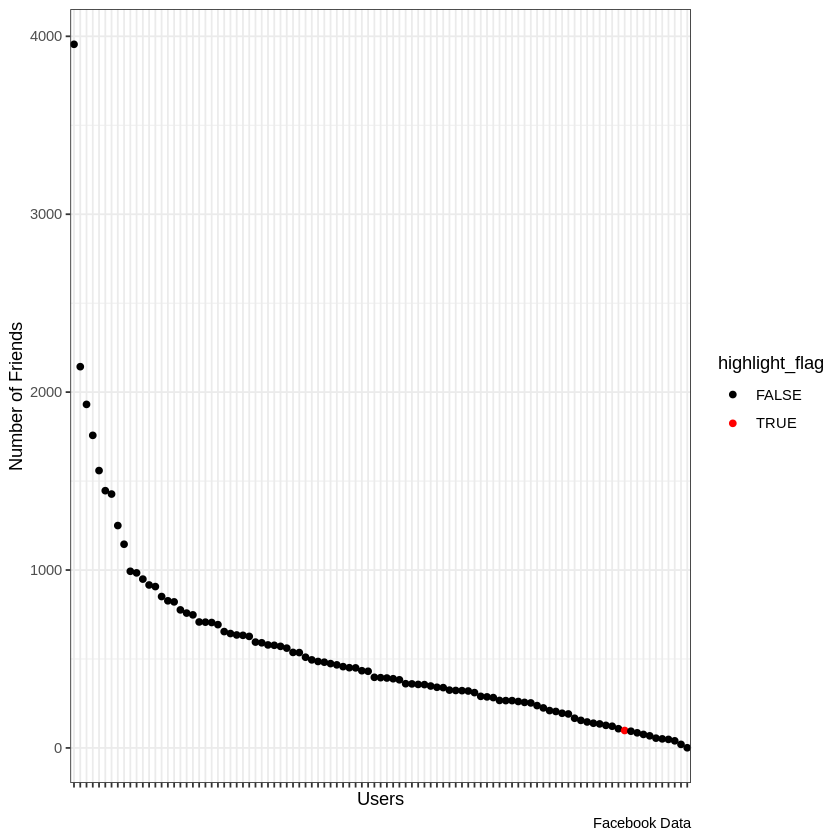
\includegraphics[width=\textwidth] {facebookGraph.png}
    \caption{Facebook friends graph.}
    \label{friendsGraph}
\end{figure}

\subsection*{Discussion}
Let's start with the data in listing \ref{facebookData}.  This was calculated by the R script in listing \ref{calFbData}, and the output was directed to ``facebookData.txt'' at the command line.  While the question does not ask for it, I felt in necessary to include the number of friends the user has by outputting the number of rows in the csv file using the ``nrow'' function.

Next is the Rscript in listing \ref{graphFriends}.  The first thing of note is the inclusion of the ``tidyverse'' library.  This library allowed me to pipe my dataset into the ``ggplot'' function.  The next thing of note is the ``theme\_update'' function that makes the x-axis blank.  You may be asking yourself ``Well how did he label the user with a blank x-axis?''  Don't worry, I'm about to answer that.  Before the data reaches the ``ggplot'' function, it is first piped through the ``mutate'' function.  Normally, ``mutate'' is used to add data, but I used it to highlight data.  In this instance, I used it to highlight the user.  To do this, I had to add the user to the data set.  I manually (using vim) added the user as ``U,'' as well as their friend count into a separate copy of the ``HW4-friend-count.csv'' file called ``user-HW4-friend-count.csv.''  In this particular implementation, the mutate function checks to see if the user is ``U.''  If it is, then the user is highligted on the graph.  The default color scheme of the highlight flag is blue-TRUE and pink-FALSE.  I changed it on line 16 to red and black, respectively.  This means that the user is the red dot on the graph, and their friends are the black dots.

To conclude this question, it seems that the friendship paradox does hold true for this user.  Most of the user's friends have more friends than they do.


\section*{Q2}

\subsection*{Answer}

\lstinputlisting[language=Python, caption=Python script used to get follower data for weiglemc and output to ``Followers.csv.'', label=getFollowers]{getFollowers.py}

\lstinputlisting[caption=Mean standard deviation and median of Twitter followers found in Followers.csv., label=twitterData]{twitterData.txt}

\lstinputlisting[language=R, caption=R script used to calculate output in listing \ref{twitterData}., label=calTwData]{followerData.R}

\lstinputlisting[language=Python, caption=Python script to append the user and their follower count to ``user-Followers.csv.'', label=appenduser]{appendUser.py}

\lstinputlisting[language=R, caption=R script used to graph Twitter followers based on their follower count., label=graphFollowers]{graphFollowers.R}

\emph{The graph for this question is figure \ref{followersGraph}}.  It is found of page 7.

\begin{figure}[h]
    \centering
    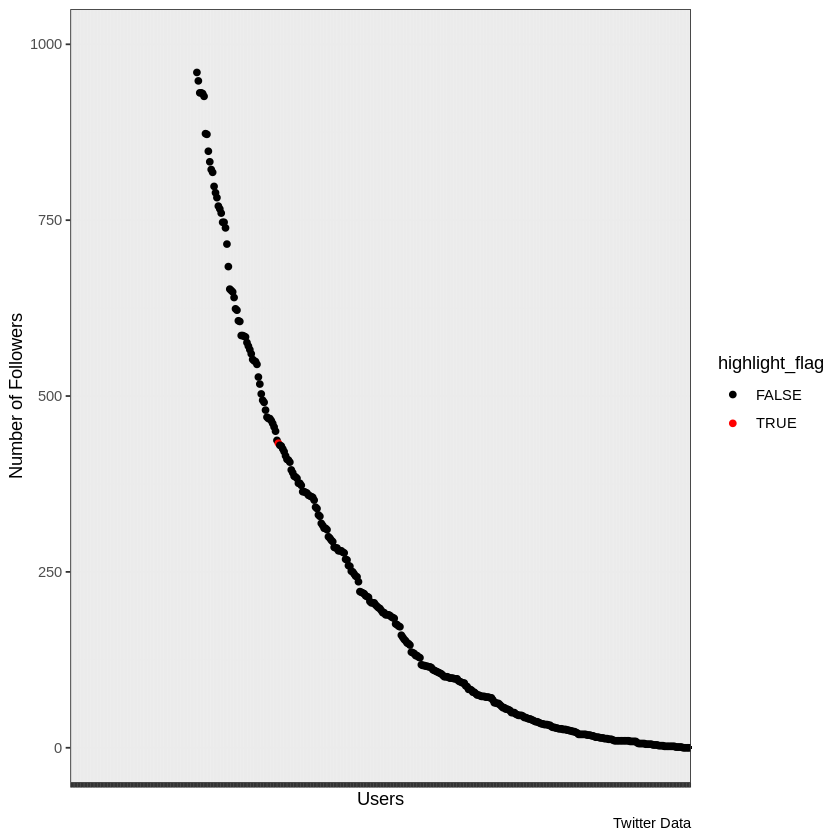
\includegraphics[width=\textwidth] {twitterGraph.png}
    \caption{Twitter followers graph.}
    \label{followersGraph}
\end{figure}

\subsection*{Discussion}
I had to use the account ``weiglemc'' to get follower data as my account has less than fifty followers.  Most of the methods used in Question 1 are used here, with some differences:

\begin{itemize}
    \item I used the Python script in listing \ref{getFollowers} to get follower data for this question.
    \item I wrote the ``Followers.csv file with a tab delimiter.
    \item Output from listing \ref{calTwData} was directed to ``twitterData.txt'' at the command line.
    \item In order to append the user to the ``user-Followers.csv'' I wrote the Python script in listng \ref{appenduser}.
    \item Because some of weiglemc's followers had so many followers, I limited the y-axis to 1,000 on line 16 in listing \ref{graphFollowers}.  This means that only users 1,000 and fewer followers appear on the graph.
    \item According to Rstudio and Google Collab, 88 rows of data do not appear in figure \ref{followersGraph}.  This means that 88 of weiglemc's followers had more than 1,000 followers.
\end{itemize}

Given that ``mweigle'' is in the top fifty percent of the ordered users in figure \ref{followersGraph}, it would seem that the friendship paradox does not hold here.


\section*{References}



\begin{itemize}
    \item{Tweepy Introduction, \url{http://docs.tweepy.org/en/latest/getting_started.html#introduction}}
    \item{Tweepy API Reference, \url{http://docs.tweepy.org/en/latest/api.html#API.followers}}
    \item{Tweepy Cursor Tutorial, \url{http://docs.tweepy.org/en/latest/cursor_tutorial.html}}
    \item{tweepy count limited to 200?, \url{https://stackoverflow.com/questions/23460560/tweepy-count-limited-to-200}}
    \item{Tweet.py search method does not support pagination, \url{https://github.com/tweepy/tweepy/issues/1040}}
    \item{Getting this error when using Tweepy, \url{https://stackoverflow.com/questions/38775997/getting-this-error-when-using-tweepy}}
    \item{Python CSV, \url{https://www.programiz.com/python-programming/csv}}
    \item{How to Write R Script Explained with an Awesome Example, \url{https://dzone.com/articles/how-to-write-r-script-explained-with-an-awesome-ex#:~:text=How\%20to\%20Create\%20R\%20Script\%201\%20You\%20can,file\%20extension\%20to\%20the\%20file.\%20More\%20items...\%20}}
    \item{Printing and displaying strings, \url{https://riptutorial.com/r/example/1221/printing-and-displaying-strings}}
    \item{R - Mean, Median and Mode, \url{https://www.tutorialspoint.com/r/r_mean_median_mode.htm}}
    \item{R Documentaion-sd, \url{https://www.rdocumentation.org/packages/stats/versions/3.6.2/topics/sd}}
    \item{The Number of Rows/Columns of an Array, \url{https://stat.ethz.ch/R-manual/R-devel/library/base/html/nrow.html}}
    \item{ggplot2 axis ticks : A guide to customize tick marks and labels, \url{http://www.sthda.com/english/wiki/ggplot2-axis-ticks-a-guide-to-customize-tick-marks-and-labels}}
    \item{How to Set Axis Limits in ggplot2, \url{https://www.statology.org/set-axis-limits-ggplot2/#:~:text=Often\%20you\%20may\%20want\%20to\%20set\%20the\%20axis,the\%20lower\%20and\%20upper\%20limit\%20of\%20the\%20y-axis.}}
    \item{How to highlight data in ggplot2, \url{https://www.sharpsightlabs.com/blog/highlight-data-in-ggplot2/#:~:text=There\%20are\%20a\%20few\%20ways\%20to\%20change\%20the,the\%20variable\%20we\%20mapped\%20to\%20the\%20fill\%20aesthetic.}}
    \item{Week-03-InfoVis-R Collab Notebook, \url{https://colab.research.google.com/github/cs432-websci-fall20/assignments/blob/master/432_Week_03_InfoVis_R.ipynb}}
    
    \end{itemize}

\end{document}

